\chapter{Range-Based Methods for High-Frequency Data} \label{chapter:2}

Wider availability of tick-by-tick/bid-ask financial transaction data has motivated the development of models that utilize this information to better estimate asset volatility. We focus on an approach which collapses high-frequency intraperiod transaction information in the form of recorded maximum and minimum prices. Work in this direction includes that of \cite{alizadeh2002range}, which uses only the range of an asset over a sampling period to extract latent stochastic volatility, while \cite{lildholdt2002estimation} uses open, high, low, and close data to do maximum likelihood estimation in a GARCH framework. \cite{rodriguez2012} combine the use of open, high, low, and close data with a Bayesian approach to estimation and prediction in a stochastic volatility framework. 
%Realized volatility demands the use of all intraperiod returns to estimate volatility. High-frequency data might not be available (due to data access), and even if available, for short periods, intraperiod returns are affected by mictrostructure noise. For short periods there might also be multiple subsequent observations recording no change in price levels. For these reasons, we are seeking an alternative estimator of volatility with high-frequency data.

\section{Problem Formulation}
Following the approach of \cite{rodriguez2012}, we are interested in finding the joint probability density for the closing, maximum, and minimum prices for an asset during a nominal period $(t-1, t)$. 
%Similarly to \cite{alizadeh2002range}, we use the range of the asset price over a trading period $\Delta$ to better estimate the volatility of the diffusion process. However, instead of just using the range of the price, we also use the opening and closing price over the interval of interest. We can let $\Delta = 1$ nominally, so that the proceeding model is defined on a period $(t-1, t)$. 
Recall the GBM model discussed in Section \ref{section:GBM}. Assuming that $\sigma$ and $\mu$ are constant over the period of interest, the log-price follows the SDE
\begin{equation}
	dY_s = \mu ds + \sigma dW_s, \label{eq:SDE}.
\end{equation}

Using the Fokker-Planck Equation, we can take the SDE in (\ref{eq:SDE}) and express the probability density of the asset price $q(y,s)$ as the PDE
\begin{eqnarray}
	\frac{\partial}{\partial s} q(y,s) &=& -\mu \frac{\partial}{\partial y}q(y,s) + \frac{1}{2}\sigma^2 \frac{\partial^2}{\partial y^2} q(y,s),  \label{eq:IV-1} \\
	q(y,t-1) &=& \delta(y-y_{t-1}), \label{eq:IV-2}
\end{eqnarray}
where $y_{t-1}$ is the price at the beginning of the interval and $\delta$ is the Dirac delta function.

The value $q(y,t)$ is the probability that $Y_t = y$, namely that the log-price of the asset is $y$ at the end of the time interval. Without any additional restrictions, therefore, the solution to the initial value problem (\ref{eq:IV-1}) - (\ref{eq:IV-2}) constitutes the likelihood of a closing price, given the parameters $\mu$ and $\sigma$, at time $s$.

Now we can incorporate the information for the high and low prices within our model if we restrict the stochastic process so it does not go below or above a certain range:
\begin{eqnarray}
	dY_s &=& \mu ds + \sigma dW_s, \label{eq:SDE-bc-1} \\
	a_t < &Y_s& < b_t. \label{eq:SDE-bc-2}
\end{eqnarray}
Equivalently, we can consider the initial value/boundary condition problem, where the boundary conditions correspond to the process having zero probability of going beyond $a_t$ and $b_t$:
\begin{eqnarray}
	\frac{\partial}{\partial s} q(y,s) &=& -\mu \frac{\partial}{\partial y}q(y,s) + \frac{1}{2}\sigma^2 \frac{\partial^2}{\partial y^2} q(y,s),  \label{eq:IV-BC-1} \\
	q(y,t-1) &=& \delta(y-y_{t-1}), \label{eq:IV-BC-2} \\
	q(a_t,s) = 0, && q(b_t, s) = 0. \label{eq:IV-BC-3} 
\end{eqnarray}

The problem in (\ref{eq:IV-BC-1}) - (\ref{eq:IV-BC-3}) can be further simplified by a transformation which eliminates the first derivative term, thereby transforming the advection-diffusion problem to a purely diffusion problem. Letting 
\begin{equation}
	q(y,s) = \exp(ay + bs)p(y,s), \label{eq:q}
\end{equation}
we apply the spatial differential operator and the time-derivative to the right side of equation (\ref{eq:q}) and equate the two expressions. We thus obtain the differential equation

\begin{equation}
 p(y,s)\left[ -\mu a + \frac{1}{2}\sigma^2 a^2 \right] + \frac{\partial}{\partial y} p(y,s)\left[ -\mu + \frac{1}{2}\sigma^2 a \right] + \frac{\partial^2}{\partial y^2} p(y,s) \left[ \frac{1}{2}\sigma^2 \right] = bp(y,s) + \frac{\partial}{\partial s}p(y,s) 
\end{equation}

The system 
\begin{eqnarray}
	-\mu a + \frac{1}{2}\sigma^2 a^2 &=& 0 \label{eq:a} \\
	b &=& 0 \label{eq:b}
\end{eqnarray}
defines $a = \sqrt{2\mu}/\sigma$, and $b=0$ such that the original problem is reduced to the heat equation on a bounded domain, with the same IC/BV conditions:
\begin{eqnarray} 
\frac{\partial}{\partial s}p(y,s) &=& \frac{1}{2}\sigma^2 \frac{\partial^2}{\partial y^2} p(y,s)  \label{eq:heat1} \\
					p(y,s) &=& 0, \qquad \qquad \quad \mbox{for}  \quad y = a_t, b_t \label{eq:heat2} \\
					p(y,0) &=& \delta(y-y_{t-1})  \label{eq:heat3}
\end{eqnarray}

%Letting $M_t = \sup_{s \in (t-1,t)}\{ Y_s \}$ and $m_t = \inf_{s \in (t-1,t)}\{ Y_s \}$, the solution to the IV/BV problem is the probability  
%\[ q(y,t) = P( m_t \geq a_t, M_t \leq b_t, Y_t = y | Y_{t-1} = y_{t-1}, m_t < M_t ). \]

%In further using this likelihood for variance estimation, we will assume that the true minimum and maximum prices over the period $(t-1, t)$ are the observed minimum and maximum prices and set them to $a_t$ and $b_t$, respectively. There are two problems with this assumption. First, even under a high frequency sampling, the prices are observed discretely so that the true maximum price is greater than $b_t$ and the true minimum price is less than $a_t$. Second, as sampling frequency increases, microstructure noise becomes more prominent. These two problems will be disentangled later. 

%The above probability is a cumulative density with respect to the boundary values. Hence, the probability density function for the boundary values and closing price is obtained by differentiating twice with respect to $a_t$ and $b_t$
%\begin{equation}
 %-\frac{\partial^2 }{\partial a_t \partial b_t } q(y,t) = P( m_t = a_t, M_t = b_t, Y_t = y | Y_{t-1} = y_{t-1}, m_t < M_t )  \label{eq:likelihood}
%\end{equation}

%This PDF is very important, as its maximization over the parameters $\mu$ and $\sigma$ produces maximum likelihood estimates $\hat{\mu}$ and $\hat{\sigma}$, which incorporate the max/min information over the period $(t-1, t)$. MLE estimates are consistent and efficient, so that the estimators based on the solution to the IV/BV problem will outperform other ad-hoc range-based estimators in the presence of more data. The current approach to estimating volatility, if microsctructure noise is temporarily ignored, is suitable for high-frequency data, because the observed maximum and minimum over a given period approach the true extrema of the prices as sampling frequency increases. 

\subsection{Closed-Form Solution to the IV/BV Problem via Fourier Expansion}

The Strum-Liouville problem in (\ref{eq:heat1}) - (\ref{eq:heat3}) can be solved by recognizing that the solution is separable. By treating the temporal and spatial differential equations independently, the solution to the problem takes on the familiar Fourier series expansion, except the coefficients of the trigonometric terms decay with time
\begin{equation}
	p(y,s) = \sum_{n=1}^\infty C_{n} \exp\left( -\lambda_n s \right) \sin\left( \frac{n\pi (y- a_t)}{b_t - a_t} \right). \label{eq:trig-expansion}
\end{equation}
There are no cosine terms in the expansion as they do not satisfy the boundary conditions. The expression for $\lambda_n$ is found by substituting the solution into the governing system of equations (\ref{eq:heat1}) - (\ref{eq:heat3}) and, after cancellation, 
\[
	\lambda_n = -\frac{1}{2}\sigma^2 \frac{n^2 \pi^2}{(b_t - a_t)^2}
\]

The coefficients $\left\{ C_n \right\}_{n=1}^\infty$ are found by first recognizing an important property of the sine-series expansion of the solution, the orthogonality of the basis functions with respect to an inner product. Defining $\xi = y - a_t$ and $L = b_t - a_t$, the inner product of two functions $h(\xi)$ and $g(\xi)$ is given by $\int_{0}^L h(\xi)g(\xi) d\xi$. The orthogonality is demonstrated by the inner product of two basis functions:
\[
	\int_0^L \sin\left( \xi \frac{n\pi}{L} \right) \sin\left( \xi \frac{m\pi}{L} \right) d\xi =\frac{1}{2} \int_0^L \cos\left( \xi \frac{(n-m)\pi}{L} \right) - \cos\left( \xi \frac{(n+m)\pi}{L} \right) d\xi = \left\{ \begin{array}{cc}
														0 & \mbox{ if } n \neq m \\
														L/2 & \mbox{ if } n = m
													\end{array}
													\right.
\]
Next, we consider the initial condition with $s=0$
\[ p(\xi,0) = \sum_{n=1}^\infty C_n \sin\left( \xi \frac{n\pi}{L} \right) = \delta(\xi - (y_{t-1}-a_t) ). \]
Using the orthogonality condition,
\[
	 \int_0^L p(\xi,0) \sin\left( \xi \frac{n' \pi}{L} \right) d\xi = \sum_{n=1}^\infty C_n \int_0^L \sin\left( \xi \frac{n' \pi}{L} \right) \sin\left( \xi \frac{n \pi}{L} \right) d\xi  = C_{n'} \frac{L}{2}.
\]
Substituting the initial condition,
\[
	\int_0^L p(\xi,0) \sin\left( \xi \frac{n' \pi}{L} \right) d\xi = \int_0^L \delta(\xi - (y_{t-1} - a_t)) \sin\left( \xi \frac{n' \pi}{L} \right) d\xi = \sin\left( (y_{t-1} - a_t) \frac{n' \pi}{L} \right)
\]
From the two conditions, we have a form for the coefficients:
\begin{equation}
	C_{n'} = \frac{2}{L} \sin\left( (y_{t-1} - a_t) \frac{n' \pi}{L} \right)
\end{equation}
Thus, the final form for $p$ is 
\begin{equation}
	p(y,s) = \sum_{n=1}^\infty \frac{2}{L} \sin\left( (y_{t-1} - a_t) \frac{n \pi}{L} \right) \exp\left( -\frac{1}{2}\sigma^2 \frac{n^2 \pi^2}{L^2} s \right) \sin\left( (y-a_t) \frac{n\pi}{L} \right) \label{eq:p}
\end{equation}

Combining equations (\ref{eq:q}), (\ref{eq:a})-(\ref{eq:b}), and (\ref{eq:p}), final solution to the IV/BC problem is
\begin{equation}
	q(y,s) = \exp\left( \frac{\sqrt{2\mu}}{\sigma} y \right) \sum_{n=1}^\infty \frac{2}{L} \sin\left( (y_{t-1} - a_t) \frac{n \pi}{L} \right) \exp\left( -\frac{1}{2}\sigma^2 \frac{n^2 \pi^2}{L^2} s \right) \sin\left( (y-a_t) \frac{n\pi}{L} \right) \label{eq:q-final}
\end{equation}

\subsection{Closed-Form Solution to the IC/BV Problem via Method of Images}
An alternative way to solve the diffusion problem in equations (\ref{eq:heat1}) - (\ref{eq:heat3}) is through the Method of Images. The general idea of the method is to find the fundamental solution to the IC problem in equations (\ref{eq:heat1}) and (\ref{eq:heat3}). For convenience of mathematical notation, we study time evolution from $t$ to $t+1$. The initial value is then $y(0) = y_t$. We enforce the boundary conditions through an appropriate series of reflections. This solution can also be derived probabilistically through the reflection principle for Brownian motion, as given by \cite{freedman1971brownian}.

The solution to the initial condition problem in equations (\ref{eq:heat1}) and (\ref{eq:heat3}) is the Green's function for the heat equation, which is known to be pdf of the Normal distribution with mean $y_{t-1}$ and standard deviation $\sigma \sqrt{s}$:
\begin{equation}
	g_0(y,s) = \frac{1}{\sqrt{2\pi s \sigma^2}} \exp\left( -\frac{1}{2} \frac{(y-y_t)^2}{s\sigma^2} \right) \equiv N(y; y_t, s\sigma^2) \label{eq:fundamental-solution}
\end{equation}

A single \textit{reflection} of the fundamental solution about the boundary point $a_t$ is defined in terms of a translation of the mean $\zeta(y) = 2a_t - y$ (since the fundamental solution is symmetric around the mean) and a negation of the function value, as shown in Figure (\ref{fig:g1}). The resultant reflection, denoted $r_0(y,s)$, satisfies the heat equation in (\ref{eq:heat1}):

\[ r_0(y,s) = -\frac{1}{\sqrt{2\pi s \sigma^2}} \exp\left( -\frac{1}{2} \frac{( y-\zeta(y_t) )^2}{s\sigma^2} \right) = -N(y; \zeta(y_t), s\sigma^2) \]

By construction, both $r_0$ and $g_0$ have the same magnitudes at $y = a_t$ but with opposing signs. The sum of the fundamental solution and its reflection, denoted as $g_1(y,s)$ and shown below in (\ref{eq:sum1}), therefore satisfies the heat equation, as well as  the boundary condition $g_1(a_t, s) = 0$. However, $g_1(y,s)$ does not necessarily satisfy the boundary condition $g_1(b_t, s) = 0$, as illustrated in Figure (\ref{fig:g1}).
%
\begin{equation} 
g_1(y,s) = g_0(y,s) + r_0(y,s) = N(y; y_t, s\sigma^2) - N(y; \zeta(y_t), s\sigma^2) \label{eq:sum1}
\end{equation}
%

%\begin{figure}
%	\centering
%	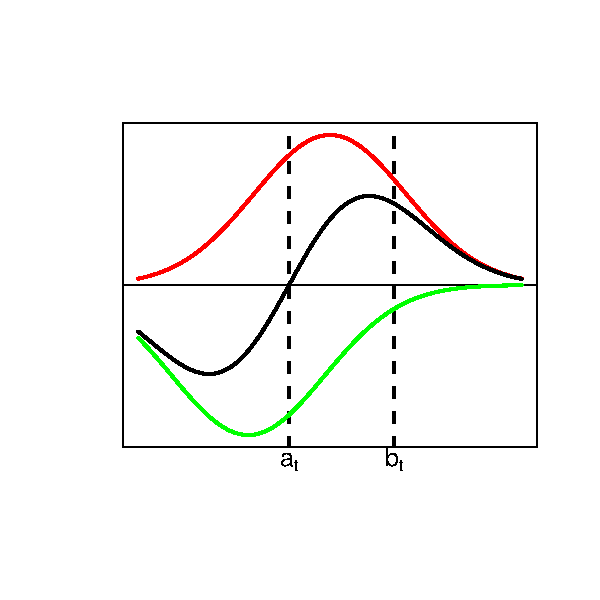
\includegraphics[scale=0.75]{g1.pdf}
%	\caption{The fundamental solution centered on $y_{t-1}$ plus a negated fundamental solution reflected about $a_t$. Here, $\sigma = 3$, $a_t = -1$ and $b_t = 1$.}
%	\label{fig:g1}
%\end{figure}

If we reflect $g_1$ about $b_t$ via a translation of the mean $\xi(y) = 2b_t - y$ and a negation:

\[ r_1(y,s) = -N(y; \xi(y_t), s\sigma^2) + N(y; \xi(\zeta(y_t)), s\sigma^2) \]

 and add this reflection to $g_1$

\[ g_2(y,s) = g_1(y,s) + r_1(y,s) = N(y; y_t, s\sigma^2) - N(y; \zeta(y_t), s\sigma^2) -N(y; \xi(y_t), s\sigma^2) + N(y; \xi(\zeta(y_t)), s\sigma^2), \] 
the resultant function $g_2$ (Figure (\ref{fig:g2})) also satisfies the heat equation and it matches the boundary condition at $b_t$, but the boundary condition at $a_t$ no longer holds. The process can be continued in this manner iteratively, with each reflection enforcing the boundary condition at $a_t$ then $b_t$. However, it is necessary to ensure that the reflections do not contain images already in the system of images.

Each reflection sends the sources of the reflected fundamental solutions further away from the domain $[a_t, b_t]$, making the maximal factor by which the boundary conditions are violated less and less. Thus, we can write down the solution to the IC/BV problem as the infinite sum of the superposition of reflected fundamental solutions. This can be defined by all possible alternating combinations of $\xi$ and $\zeta$ applied to the center of $g_0$. The expression in (\ref{eq:images}) enumerates all such combinations and is therefore the solution to the diffusion equation under the initial conditions and boundary values. 
%
\begin{align}
	p(y,s) &= N( y ; y_{t-1}, s\sigma^2) - N( y ; \zeta(y_{t-1}), s\sigma^2) - N( y ; \xi(y_{t-1}), s\sigma^2) + \nonumber \\
		& \quad \sum_{n=1}^\infty \left[ N( y ; (\xi \circ \zeta)^n (y_{t-1}), s\sigma^2) + N(y ; (\zeta \circ \xi)^n (y_{t-1}), s\sigma^2 ) \right. \nonumber \\
		&  \qquad \qquad \left. -  N( y ; (\xi \circ \zeta)^n \circ \xi (y_{t-1}), s\sigma^2) - N( y ; (\zeta \circ \xi)^n \circ \zeta (y_{t-1}), s\sigma^2) \right]. \label{eq:images}
\end{align}
%
The final solution to the original advection-diffusion problem is therefore $p(y,s)$ multiplied by the exponential factor $\exp(ay+bs)$, which is given in equation(\ref{eq:q-final-images}). Figure (\ref{fig:g3}) shows the solution from equation (\ref{eq:images}) with $n=1$. 

%\begin{figure}
%	\centering
%	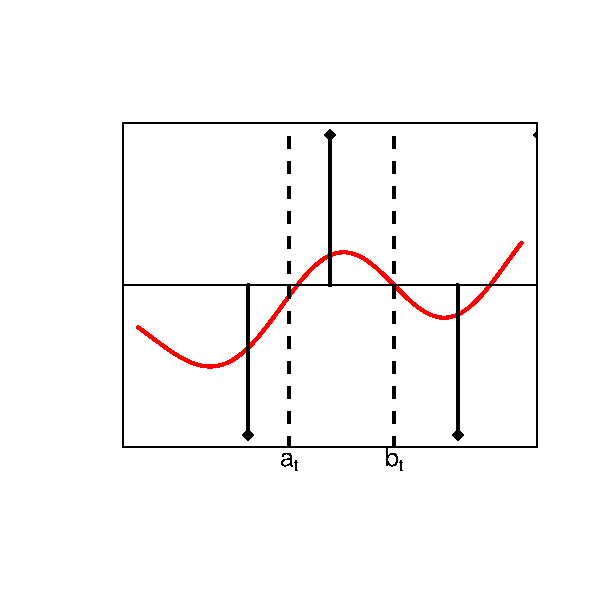
\includegraphics[scale=0.75]{g2.pdf}
%	\caption{The solution obtained by a reflection about $a_t$ then $b_t$.}
%	\label{fig:g2}
%\end{figure}

%\begin{figure}
%	\centering
%	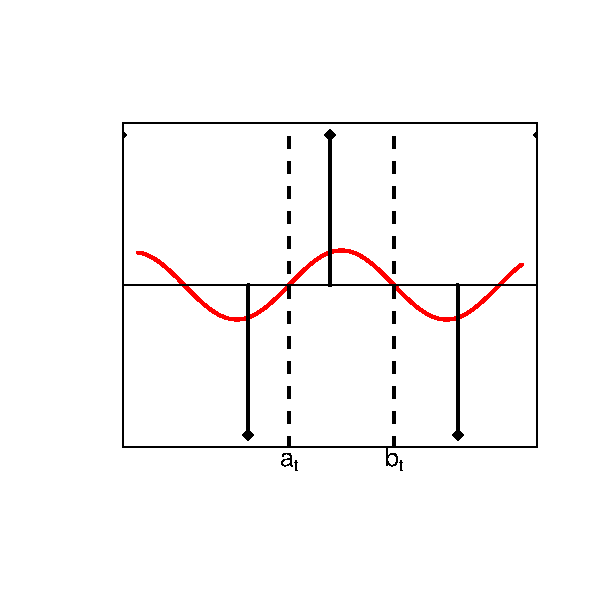
\includegraphics[scale=0.75]{g3.pdf}
%	\caption{The solution obtained by a reflection about $a_t$ then $b_t$.}
%	\label{fig:g3}
%\end{figure}

\begin{figure}[htbp]
        \centering
        \begin{subfigure}[t]{0.3\textwidth}
                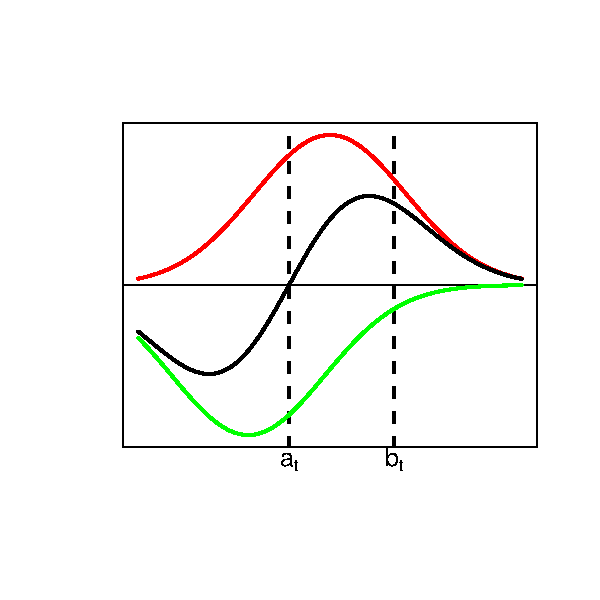
\includegraphics[width=\textwidth]{g1.pdf}
                \caption{The fundamental solution $g_0$ (red), its reflection about $a_t,$ $r_0$ (green), and their sum $g_1$ (black). Observe that the boundary condition is satisfied at $a_t$ but not $b_t$.}
                \label{fig:g1}
        \end{subfigure}%
        ~ %add desired spacing between images, e. g. ~, \quad, \qquad, \hfill etc.
          %(or a blank line to force the subfigure onto a new line)
        \begin{subfigure}[t]{0.3\textwidth}
                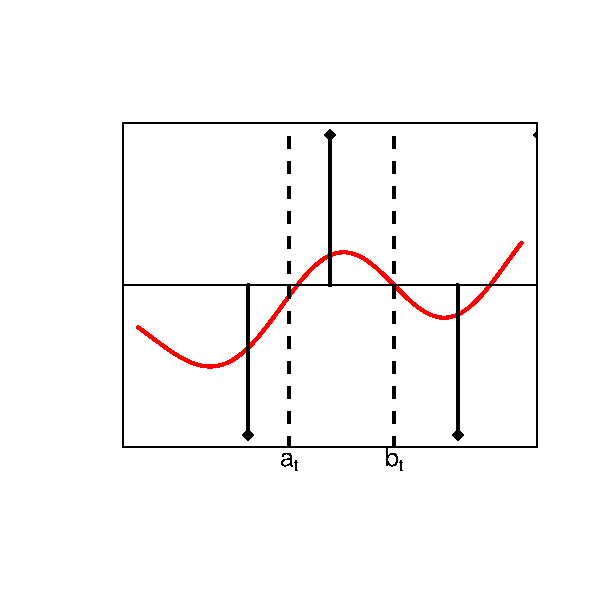
\includegraphics[width=\textwidth]{g2.pdf}
                \caption{The solution after a single reflection about $a_t$, $g_1$ (red), its reflection about $b_t$, $r_1$ (green), and their sum $g_2$ (black). The boundary condition is satisfied at $b_t$ but is now violated at $a_t$.}
                \label{fig:g2}
        \end{subfigure}
        ~ %add desired spacing between images, e. g. ~, \quad, \qquad, \hfill etc.
          %(or a blank line to force the subfigure onto a new line)
        \begin{subfigure}[t]{0.3\textwidth}
                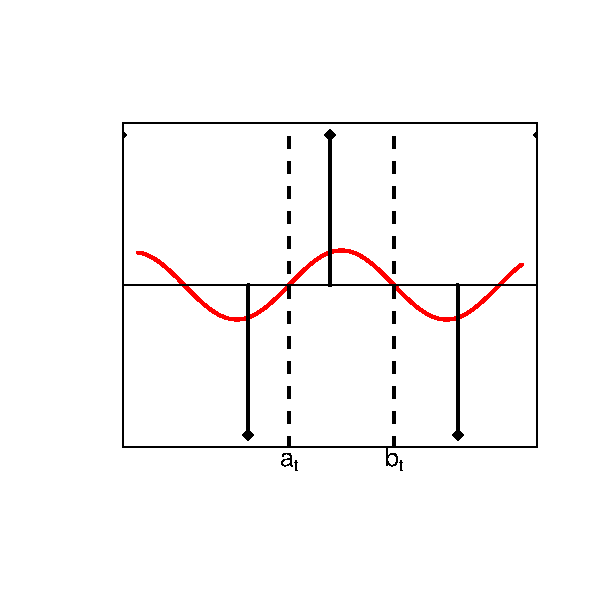
\includegraphics[width=\textwidth]{g3.pdf}
                \caption{The solution according to equation (\ref{eq:images}) with $n=1$. }
                \label{fig:g3}
        \end{subfigure}
        \caption{Construction of the solution using the Method of Images}\label{fig:animals}
\end{figure}

\begin{eqnarray}
	q(y,s) &=& \exp\left( \frac{\sqrt{2\mu}}{\sigma} y \right) \times \nonumber \\
		&& \Bigg\{ N( y ; y_{t-1}, s\sigma^2) - N( y ; \zeta(y_{t-1}), s\sigma^2) - N( y ; \xi(y_{t-1}), s\sigma^2) + \nonumber \\
		&& \quad \sum_{n=1}^\infty \left[ N( y ; (\xi \circ \zeta)^n (y_{t-1}), s\sigma^2) + N(y ; (\zeta \circ \xi)^n (y_{t-1}), s\sigma^2 ) \right. \nonumber \\
		& & \qquad \left. -  N( y ; (\xi \circ \zeta)^n \circ \xi (y_{t-1}), s\sigma^2) - N( y ; (\zeta \circ \xi)^n \circ \zeta (y_{t-1}), s\sigma^2) \right] \Bigg\} . \label{eq:q-final-images} 
\end{eqnarray}

%the above partial differential equation becomes
%\[ \Phi'(s)f(y) = \frac{1}{2}\sigma^2 \Phi(s) f''(y) \]
%Isolating functions of $s$ and $y$, we see that the ratios of the solution functions and their respective derivatives must be equal to a constant independet of the two variables
%\[ \frac{\Phi'(s)}{\Phi(s)} = \frac{1}{2}\sigma^2 \frac{f''(y)}{f(y)} = \frac{1}{\lambda}. \]
%The solution to the time-dependent problem is $\Phi(s) = \Phi(0)\exp(\lambda t)$. For the solution to be defined over all $t$, we need $\lambda < 0$. The spatial problem, a second-order linear differential equation 
%\[ f''(y) = \frac{2}{\sigma^2 \lambda} f(y) = -\frac{2}{\sigma^2 |\lambda|} f(y) \]
%is satisfied by the linear combination
%\[ f(y) = A\sin\left( y\sqrt{\frac{2}{\sigma^2 |\lambda| }} \right) + B\cos\left( y\sqrt{\frac{2}{\sigma^2 |\lambda| }} \right), \]
%where we require at least one of $A$ and $B$ be nonzero. In addition to satisfying the differential equation, $f(y)$ must also satisfy the boundary contions. Hence,
%\begin{eqnarray*}
%	f(a_t) &=&  A\sin\left( a_t\sqrt{\frac{2}{\sigma^2 |\lambda|}} \right) + B\cos\left( a_t\sqrt{\frac{2}{\sigma^2 |\lambda|}} \right) = 0, \\
%	f(b_t) &=&  A\sin\left( b_t\sqrt{\frac{2}{\sigma^2 |\lambda|}} \right) + B\cos\left( b_t\sqrt{\frac{2}{\sigma^2 |\lambda|}} \right) = 0. 
%\end{eqnarray*}
%
%We can re-scale the problem by a shift of $a_t$ so that $a_t \to 0$ and $b_t \to b_t - a_t \equiv L$. Let $\xi \equiv y - a_t$. Under this transformation, we have 
%\begin{eqnarray*}
%	B &=& 0, \\
%	A\sin\left( L\sqrt{\frac{2}{\sigma^2 |\lambda|}} \right) + B\cos\left( L\sqrt{\frac{2}{\sigma^2 |\lambda|}} \right) &=& 0. 
%\end{eqnarray*}
%Therefore, $B=0$, which forces $A \neq 0$. It follows that $\sin\left( L\sqrt{\frac{2}{\sigma^2 |\lambda|}} \right) = 0$, which means that
%\[ L\sqrt{\frac{2}{\sigma^2 |\lambda|}}  = n\pi, \quad n=1, \ldots \quad ( n \neq 0 \mbox{ because } L \neq 0 ) \]
%Since $n$ goes over the integers, there is a countable number of constants, or \textit{modes}, $\lambda_n$ for our problem, given by
%\[ \lambda_n = -\frac{2L^2}{n^2 \pi^2 \sigma^2 }. \]
%Thus, the solution to the problem, both in time and space, is given by the sum of basis functions for each mode
%\[ p(\xi, t) = \sum_{n=1}^\infty \Phi_n(t) f_n(\xi ) = \sum_{n=1}^\infty \Phi_n(0) \exp\left( -\frac{2L^2}{n^2 \pi^2 \sigma^2 } t \right) A_n \sin\left( \xi \sqrt{\frac{2}{\sigma^2 \frac{2L^2}{n^2 \pi^2 \sigma^2 }}} \right) = \sum_{n=1}^\infty \tilde{A}_n \exp\left( -\frac{2L^2}{n^2 \pi^2 \sigma^2 } t \right) \sin\left( \xi \frac{n\pi}{L} \right). \]
%Expressing the solution in terms of $y$ instead of $\xi$,
%\[ p(y,t) =  \sum_{n=1}^\infty \tilde{A}_n \exp\left( -\frac{2L^2}{n^2 \pi^2 \sigma^2 } t \right) \sin\left( (y-a_t) \frac{n\pi}{L} \right). \]

%There are a few things that must be observed of this solution. First, the constants $\Phi_n(0)$ and $A_n$ have been combined into $\tilde{A}_n$, which is determined by the sine series representation for the initial condition, $\delta(y - y_t)$. This will be dealt with below. Second, the contribution of each additional mode decays at the order of $\exp(-1/n^2)$, making the approximation of $p(y,t)$ in terms of a finite number of terms very efficient. Finally, the solution behaves as expected: $p(y,t) \to 0$ as $t \to \infty$. This corresponds to the intuition that as time progresses a particle is less likely to stay bounded between the values $a_t$ and $b_t$. 


\section{Finding the Likelihood for the Closing Price}
The full solution $q(y,t)$ is the likelihood that a random process satisfying the stochastic differential equation (\ref{eq:SDE}) has an infimum greater than or equal to $a_t$ and a supremum less than or equal to $M_t$ over the period $(t-1, t)$.  In terms of probabilities
\[
	q(y,t) = P( m_t \geq a_t, M_t \leq b_t, Y_t = y | Y_{t-1} = y_{t-1}, m_t < M_t ).
\]
%
However, to perform the statistical inference we need the density associated with $q(y,t)$, which is derived by differentiating $q(y,t)$ with respect to the boundary conditions:
\begin{equation} -\frac{\partial^2 }{\partial a_t \partial b_t } q(y,t) = P( m_t = a_t, M_t = b_t, Y_t = y | Y_{t-1} = y_{t-1}). \label{eq:likelihood}
\end{equation}
%
The analytic expression for the likelihood, whether that in equation (\ref{eq:q-final}) or (\ref{eq:q-final-images}), allows us to perform this differentiation numerically as well as analytically. Once this differentiation is performed, we can use familiar optimization methods to find maximum likelihood estimates for the parameters $\mu$ and $\sigma^2$, given closing, open, high, and low prices for a given interval $(t-1,t)$. 

\subsection{Evaluating the accuracy of the solutions}

We want to compare the convergence of the likelihood (\ref{eq:likelihood}) based on the trigonometric expansion solution (\ref{eq:q-final}). This convergence is dependent upon the number of terms used in the truncated summation for the expansion, as well as the size of the discrete step when performing numerical differentiation. This analysis sets the stage for our treatment of the bivariate advection-diffusion problem in Chapter 3.

Considered are ten simulations over a nominal period of length 1 based on a forward-Euler discretization scheme of the governing stochastic differential equation:
\begin{equation} 
	Y_{k+1} = Y_{k} + \mu \Delta t^* + \sigma \Delta t^* \epsilon_k, \label{eq:SDE-discrete}
\end{equation}
with $\Delta t^* = 1/23,400$,  and $\epsilon_k \sim N(0,1)$. This is equivalent to sampling the returns once every second over the length of a trading day. Further, 
\[ \mu = 1, \qquad \sigma = 1. \]
For each simulation there is a recorded min, max, and closing value, while all log open prices are set to 0. As a test to study the numerical accuracy of the solution, we examine the likelihood value at the closing log return using the observed minima and maxima set to $a_t$ and $b_t$ respectively, as well as the true $\mu$ and $\sigma$ used to generate the data. When performing numerical differentiation, a second-order two-point stencil method is used with a discretization step
\[ 
	\Delta x = \frac{1}{2^k} \frac{1}{100} (b_t - a_t).
\]
Values of the likelihoods are considered across ranges of $N$ and $k$ and are compared to the likelihood values obtained through analytic differentiation. The results are shown in Tables (\ref{table:m4}) - (\ref{table:analytic}). We see that for both numerical differentiation factors $k=4$ and $k=8$ likelihood values match with those obtained via analytic differentiation, so either differentiation approach is appropriate for maximum likelihood estimation. Further, we see that likelihood values are the same across all sizes of $N$. This means that the number of terms needed in the trigonometric expansion for accurate solutions is relatively low, and the Fourier expansion used in our derivation is an efficient representation for the univariate diffusion problem.

\begin{table}
	\centering
	\csvautotabular{./chapter-2-univariate-case/table-m-4.csv}
	\caption{Likelihood values for simulations obtained via numerical differentiation with $k=4$ ($\Delta x = 1/(100 \cdot 2^4) \cdot (b_t-a_t)$). }
	\label{table:m4}
\end{table}

\begin{table}
	\centering
	\csvautotabular{./chapter-2-univariate-case/table-m-8.csv}
	\caption{Likelihood values for simulations obtained via numerical differentiation with $k=8$ ( $\Delta x = 1/(100 \cdot 2^8) \cdot (b_t-a_t)$). }
	\label{table:m8}
\end{table}

\begin{table}
	\centering
	\csvautotabular{./chapter-2-univariate-case/table-analytic.csv}
	\caption{Likelihood values for simulations obtained via analytic differentiation. }
	\label{table:analytic}
\end{table}


\section{Using Close, High, Low, Open Data for High-Frequency Data: a Monte Carlo Simulation Study}
For high-frequency data where transactions occur on the microsecond scale, there is a lot of available information even within sampling intervals on the second scale. Realized volatility estimates use all data within sampling intervals, while the estimates based on the likelihood developed above use summaries of intraperiod data in the form of open, close, high, and low (OCHL) recorded prices. In this simulation study, we are interested in seeing how our maximum likelihood estimates for $\sigma^2$ based on OCHL data compare with RV estimates.

%Discussed previously was the Realized Volatility estimator, which is a model-free estimator for the integrated volatility of a process over an interval $\Delta$. In the absence of microstructure noise, we know that $RV \to \int_{t-1}^t \sigma^2(y_s,s)dW = \sigma^2$ (for a constant $\sigma^2$ over $\Delta = (t-1,t)$) as the number of samples over the interval $(t-1,t)$ goes to infinity. Precisely because of this limiting property, the RV estimator is widely used in the estimation of volatility models with high-frequency data. In addition to the standard RV estimator in equation (\ref{eq:RV}), we will consider an RV estimator which attempts to overcome the bias introduced by microsctructure noise. 
%
%We are interested in seeing how our maximum likelihood estimates for $\sigma^2$ based on open, close, high, and low (OCHL) data compare with RV estimates. We consider two simulation-based scenarios, one with and one without microstructure noise. 
%
\subsection{Maximum Likelihood Estimation}
The goal of the simulation study is to understand the trade-offs between using all high-frequency data and, instead, using summaries. Recalling the basic diffusion model in (\ref{eq:SDE}) with constant $\mu$ and $\sigma^2$, the simulations use 
\[ \mu = 7.936508 \cdot 10^{-5}, \qquad \sigma = 0.01259882. \]
The parameters correspond to daily estimates for drift and standard deviation of the returns of the S\&P 500 index. Thus, in our simulations $\Delta$ corresponds to an idealized 7-hour trading day. The simulated data is obtained by the forward-Euler discretization in equation (\ref{eq:SDE-discrete}), where $\epsilon_k \sim N(0,1)$, and index $k$ corresponds to the time $k \Delta t^* $, and $\Delta t^*$ corresponds to a second of a trading day. Generating the data according to equation (\ref{eq:SDE-discrete}) amounts to sampling the diffusion process every second. It should be noted here that the data-generation method used here does not include microstructure noise.

When performing estimation, longer sampling intervals are used. They are  
\[ \Delta t = 5 \mbox{ sec}, 10 \mbox{ sec}, 20 \mbox{ sec}, 30 \mbox{ sec}, 1 \mbox{ min}, 5  \mbox{ min}, 10 \mbox{ min}, 20 \mbox{ min}, 30 \mbox{ min}, 1 \mbox{hr}, 3.5 \mbox{hr}, 7 \mbox{hr}. \]
We expect the realized volatility estimate to approach the true diffusion parameter, in probability, as $\Delta t \to 0$. As for estimating volatility using OCHL data, each simulated day contains $1/\Delta t$ intervals. Each interval $[k\Delta t, (k+1)\Delta t]$, in turn, contains $\Delta t/\Delta t^* + 1$ data points. For example, if $\Delta t = 5\mbox{ sec}$, there are six data points in the interval $[k\Delta t, (k+1)\Delta t]$: the price observed at time $k \Delta t$, and a price every second up to, and including, time $(k+1) \Delta t$. The price at time $k\Delta t$ is the opening price, the price at time $(k+1)\Delta t$ is the closing price, and the minimum and maximum prices observed in the samples between are used as $a_t$ and $b_t$ respectively for the likelihood in (\ref{eq:likelihood}). Using this data and the analytic expression for the likelihood, we optimize over $\mu$ and $\sigma^2$ to find the maximum likelihood estimates for the parameters. Thus, for every simulated day for a given $\Delta t$, there is an independent set of estimates for $\sigma^2$ and $\mu$. 

The results for 1000 simulated trading days are shown in Figure (\ref{fig:estimator-comparison-no-microstructure}). We see that, for the shortest sampling periods, the realized volatility estimator outperforms the OCHL estimator in terms of both bias and mean-squared error, as expected. However, the variance of the RV estimator is much greater than that of the OCHL estimator. As a result, the OCHL estimator quickly overtakes the RV estimator in terms of MSE performance.

It is notable that the OCHL estimator has a large bias for small sampling periods. As long as the observations of a diffusion process are finite in number, the observed maximum is less than or equal to the true maximum and the observed minimum is greater than or equal to the true minimum. The discrepancy between the true and observed extreme values becomes greater as the number of observations becomes smaller. This artificially smaller range between extreme values biases the estimates for volatility to be below the true value for smaller intervals $[k\Delta t, (k+1)\Delta t]$ since they contain fewer data points. 

\begin{figure}
	\centering
	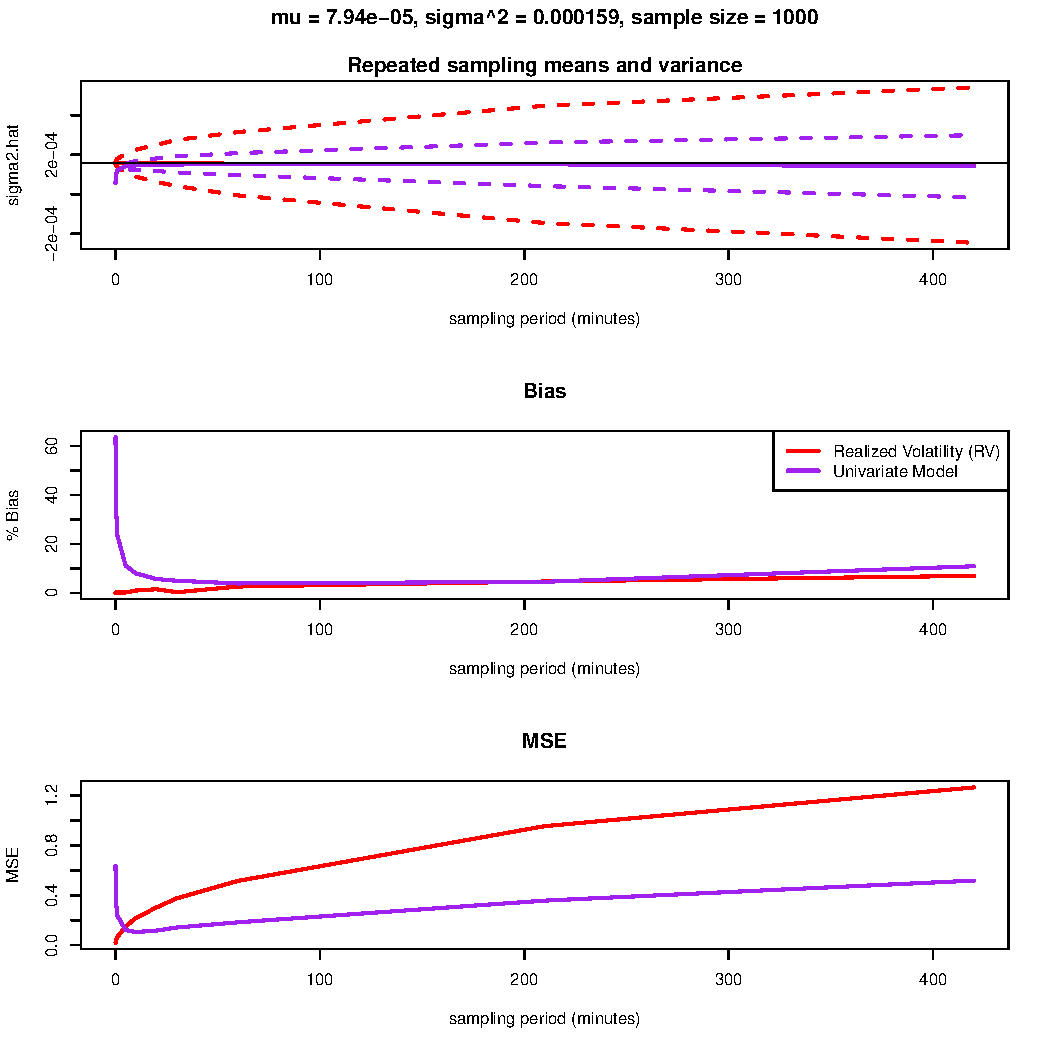
\includegraphics[scale=0.8]{results-7-14-13-5-53.pdf}
	\caption{Results for 1000 trading days}
	\label{fig:estimator-comparison-no-microstructure}
\end{figure}

%\subsection{Estimation With Microstructure Noise}
%It is important to examine how robust the RV and OCHLO estimators are to microstructure noise. The confounding phenomenon is introduced through the data generating process as an additional noise term: 
%\begin{equation} 
%	Y_{k+1} = Y_{k} + \mu \Delta t^* + \sigma \Delta t^* \epsilon_k + \gamma \nu_k, \label{eq:SDE-discrete-noise}
%\end{equation}
%with $\nu_k \sim N(0,1)$. Considered are a number of magnitudes for the noise term $\gamma$. It should be noted that the noise added to the observation does not scale with observation periods. This means that for short intervals, $\gamma$ can dominate the diffusion process, but as the sampling interval $\Delta t$ increases, $\gamma$ becomes negligible with respect to the diffusion variance $(\sigma \Delta t)^2$. This is precisely the empirical market dynamics of microstructure noise. Thus, we expect both types of estimators to perform as above for bigger $\Delta t$, but of particular interest are shorter sampling intervals. 